\documentclass[11pt, titlepage]{article}

\usepackage[utf8]{inputenc}
\usepackage[T1]{fontenc}
\usepackage{lmodern}
\usepackage[english]{babel}
\usepackage{verbatim}
\usepackage{hyperref}
\usepackage{graphicx}
\usepackage{listings}

\lstset{
basicstyle=\small\ttfamily,
inputencoding=utf8,
columns=flexible,
breaklines=true
}
\lstset{
     literate=%
         {à}{{\'a}}1
         {é}{{\'e}}1
         {è}{{\`e}}1
         {ê}{{\^{e}}}1
         {ô}{{\^{o}}}1
         {ù}{{\`u}}1            
}

\author{Auteur : REN Marc
Encadrants : ZIAT Ghiles, BOTBOL Vincent}
\newcommand{\authorLastName}{REN}
\title{Bibliothèque logicielle pour impression 3D d’objets contraints}
\newcommand{\experimentShortName}{Bibliothèque logicielle pour impression 3D d’objets contraints}

\usepackage{color}
\usepackage{sectsty}
\definecolor{WordSectionBlue}{RGB}{30, 90, 147}
\allsectionsfont{\color{WordSectionBlue}}

\begin{document}

\maketitle
\newpage
\newpage
\tableofcontents
\newpage
\section{Introduction}
L'impression 3D est le terme courant pour parler d'un procédé de fabrication additive. Ce procédé existe depuis le milieu des années 80 et connaît un certain engouement dû à la commercialisation d'imprimantes 3D destinées au grand public.
Il existe plusieurs technologies permettant cette méthode de fabrication :
le SLS ou Selective Laser Sintering, frittage sélectif par laser en français;
le SLA ou StereoLithograph Apparatus, l'impression par stéréolithographie (solidification d'une couche de plastique liquide par émission de lumière UV);
le FDM ou Fuse Deposition Modeling, modelage par dépôt de matière en fusion.
C'est cette dernière qui est la plus répandue et qui est employée par l'imprimante 3D de marque Ultimaker que nous avons utilisée tout au long de notre projet, la matière portée en fusion étant du plastique.

Une impression 3D peut se résumer à déplacer la tête d'impression, que nous appellerons extrudeur par la suite, avec ou sans dépôt de plastique, dans les limites de l'espace qui est disponible à la machine. Les dépôts successifs se solidifient et se collent à la matière précédemment présente sur le support et finissent par former l'objet convoité, d'où le procédé de fabrication additive. Le \verb&gcode& est le langage assembleur de la machine utilisée et nous permet, par le biais de différentes instructions, de contrôler et paramétrer les différents éléments la composant, notamment l'extrudeur.

Actuellement, la manière la plus courante permettant d'aboutir à l'impression d'un objet 3D souhaité est d'abord de le représenter dans un logiciel de modélisation 3D pour ensuite par le biais de différents logiciels, fournir un ensemble d'instructions en \verb&gcode& qui sera interprété par l'imprimante. Notre approche est de permettre de programmer un objet 3D en permettant de représenter une couche 2D et de permettre de la transformer et de superposer ces différents couches les unes sur les autres pour arriver à un résultat en 3D.

Nous détaillerons quelles sont les différentes étapes du schéma classique d'une impression 3D, quelles sont notre motivation et notre approche de ce domaine et comment a été réalisée cette bibliothèque logicielle.

\newpage
\section{Etat de l'art}
La manière la plus courante pour imprimer l'objet 3D désiré est d'abord de le modéliser pour ensuite en générer un fichier au format \verb&gcode&.
La procédure classique suit le schéma suivant :
\begin{center}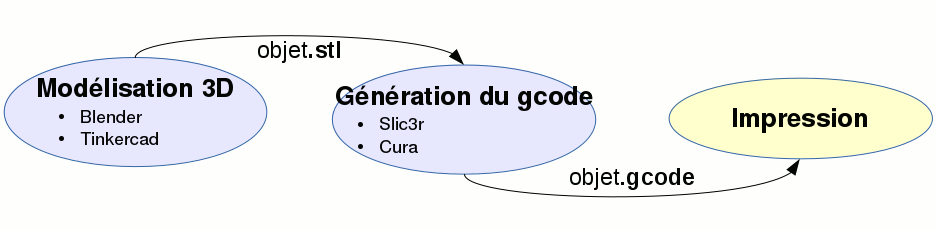
\includegraphics[scale=0.35]{img/EtatDeLart.png}\end{center}
\subsection{Modélisation}
Il existe plusieurs logiciels de modélisation 3D tels que Blender ou bien Tinkercad, tous reposant sur le même principe. Pour tous, l'idée est d'assembler dans un espace donné différents volumes ou plans jusqu'à obtenir le rendu désiré. Le modèle obtenu peut ensuite être exporté sous différents formats. Le format le plus couramment utilisé est le \verb&stl&, un acronyme pour Standard Triangle Language. Un fichier \verb&stl& décrit un objet par un ensemble de triangles, chaque triangle étant lui même décrit par trois points et d'un vecteur normal permettant de déterminer l'orientation du triangle. Plus l'objet est complexe et plus le nombre de triangles le définissant est important.

\subsection{Conversion en gcode}
Une fois l'objet modélisé et enregistré au format \verb&stl&, il est compilé au format \verb&gcode&.
Plusieurs logiciels permettent cette conversion, les logiciels les plus populaires sont Slic3r et Cura et reposent tous sur le même principe.
L'imprimante étant limitée par des contraintes physiques, la matière sortante de la tête d'impression étant solide et étant soumise à la gravité, il est impossible d'imprimer de la matière sous ce qui a déjà été sortie.
Pour obtenir le fichier \verb&gcode& correspondant à l'objet modélisé, le logiciel parcourt alors l'objet de bas en haut et le découpe en plusieurs couches horizontales dont il génère le \verb&gcode&.

\subsection{Impression}
Le fichier \verb&gcode& généré décrit une suite d'instruction ordonnée dans le même sens de parcours que le logiciel de découpe. C'est-à-dire que les instructions sont peuvent être séparés en sous-ensemble d'instructions permettant d'imprimer une couche, en commençant par la couche la plus basse jusqu'à celle la plus haute. Chaque sous-ensemble d'instructions peut paramétrer la machine et décrit le trajet que va effectuer la tête d'impression pour imprimer la couche. Ce trajet respecte certaines contraires physiques résultant du matériau utilisé. Étant donné que chaque dépôt finit par se coller à la matière déjà présente, si la tête d'impression imprime plusieurs fois au même point, ce point forme alors une irrégularité de la couche qui n'est plus lisse et dans le pire cas, à un prochain passage de la tête d'impression sur ce point, il y a un risque que celle ci déplace ou casse le résultat jusque là obtenu et compromettre le rendu final.

Ces instructions permettent de contrôler et paramétrer les différents éléments qui composent l'imprimante et dont les principaux sont des moteurs et des ventilateurs. L'un des moteurs sert à bouger la tête d'impression, que nous allons appeler par le suite extrudeur, l'axe des abscisses, un second pour bouger l'extrudeur sur l'axe des ordonnées, un troisième permettant de faire avancer ou reculer la matière à porter en fusion dans le tuyau menant à l'extrudeur et le dernier sert à bouger le support horizontal, sur lequel repose l'objet à imprimer, à la hauteur souhaitée.

\newpage
\section{Motivations et Approche}
Les logiciels de modélisation 3D, bien que très aboutis, ne permettent pas la conceptions d’objets récursifs.
L'idée du projet est de voir un objet en 3D comme étant la superposition de plusieurs couches et de proposer la possibilité d'imprimer une couche de base et les différentes transformations successives de cette couche les unes sur les autres. Ce procédé d'impression d'une couche et de ses transformations est ce que nous définissons comme étant la 2.5D, l'impression d'une couche sur l'autre permettant de donner un rendu en 3D, et nous donne une certaine garantie de la faisabilité de cet objet. Cette approche est plus proche du procédé d'impression d'un objet 3D et nous permet de déterminer si chacune des couches est imprimable, chose qui n'est pas possible lorsqu'un objet est modélisé en 3D.
En développant une bibliothèque, on souhaite donner la possibilité de programmer un objet et ainsi de doter l'impression 3D des différents outils de la programmation tels que les boucles, les structures de contrôle et autres.

Nous avons décidé que le format de sortie serait le \verb&gcode&. Cela nous permet d'avoir un contrôle plus fin de ce que fait la machine et ainsi d'avoir un résultat plus précis que ce que pourrait nous donner un logiciel de découpe d'un modèle 3D.
Par le biais de différentes séances de calibrage, nous pouvons voir comment réagit la matière portée à fusion, comment se comporte l'imprimante et les différents contraintes liées directement à la machine telle que l'espace d'impression disponible ou autres spécificités spécifiques à la machine et au matériau utilisé.
Nous pouvons aussi définir, suivant les attentes, quelle sera la qualité de l'objet obtenu en spécifiant l'épaisseur de chaque couche et de l'enveloppe extérieure de l'objet, la façon de remplir l'objet et encore d'autres paramètres jouant sur la qualité et la précision de l'objet à imprimer
Ainsi la procédure que nous proposons suit le schéma suivant :
\begin{center}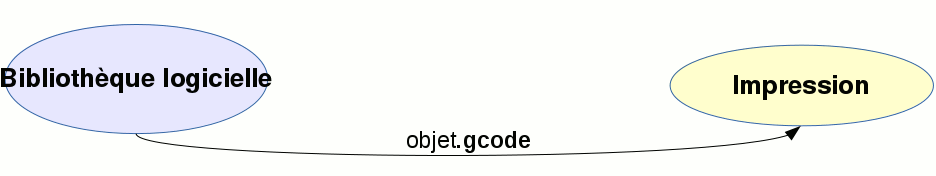
\includegraphics[scale=0.35]{img/Motivation.png}\end{center}

Cette bibliothèque est écrite en OCaml car un langage expressif, fonctionnel, fortement typé et multi-paradigme a été privilégié.

\newpage
\section{Réalisation}
L'intégralité du code est disponible sur le GitHub du projet à l'adresse suivante :
\url{https://github.com/jaunecitron/PSTL}

\subsection{Interface OCaml / gcode}
La première réalisation a donc été de créer une interface permettant de représenter les différentes instructions \verb&gcode&. Il existe deux types d'instructions, les instructions G et M. Les instructions G se numérotent de 0 à 99 et sont destinées à paramétrer et actionner tout ce qui a un lien avec la tête d'impression, que nous appellerons par la suite extrudeur; et les instructions M se numérotent de 0 à 999 et sont destinées à paramétrer les différents éléments de l'imprimante 3D autres que ceux ayant un lien avec l'extrudeur. Il y a donc potentiellement 1100 instructions possibles en plus des commentaires.
Nous avons décidé de représenter dans notre interface un sous-ensemble du jeu d'instructions. Ce sous-ensemble contient les instructions dont nous avons eu besoin et qui nous permettent d'imprimer n'importe quel objet 3D avec précision.
\newline

Ces instructions sont les suivantes :
\begin{lstlisting}
  type instruction =
  | G0 of (float * float * float * float * float * int)
  | G0_move of (float * float) (* G0(x,y) rapid move without extrude *)
  | G0_speed of (float)
  | G0_height of (float) (* G0_height(z) move to height z*)
  | G1 of (float * float * float * float * float * float)(* G1(x,y,e) move with extrude *)
  | G1_print of (float * float * float)
  | G1_speed of (float)
  | G10 of (int option) (* G10 retract *)
  | G11 of (int option) (* G11 unretract*)
  | G92_init of (float) (* G92(e) *)
  | M106_fan_speed of (int) (* M106(s) turn fan 0 at speed s *)
  | M107
  | Comment of (string)
  
  val instruction_to_string : instruction -> string
\end{lstlisting}

    \subsubsection{Déplacements linéaires, G0 et G1}
	\verb&G0(x,y,z,e,f,s)& permet de faire bouger l'extrudeur à la position (x,y,z) en faisant déplacer la matière plastique jusqu'au point e et s étant un flag signalant si l'on vérifie qu'un cas d'arrêt a été rencontré. La variante \verb&G0_move(x,y)& déplace l'extrudeur à la position (x,y), \verb&G0_speed(f)& définit la vitesse du déplacement à f mm/minutes de la commande G0 et \verb&G0_height(z)& bouge l'extrudeur à la hauteur z.
De la même façon, \verb&G1(x,y,z,e,f,s)& permet de déplacer l'extrudeur de la même façon que \verb&G0(x,y,z,e,f,s)&. La variante \verb&G1_speed(f)& a la même fonction que G0 pour la commande G1 et \verb&G1_print(x,y,e)& déplace la tête d'impression à la position (x,y) et déplace la matière plastique jusqu'au e.
L'existence de deux commandes permettant le déplacement de l'extrudeur nous permet d'en utiliser laissant un dépôt de matière et l'autre non. Nous avons dédcidé suivre les normes qui ont été définies par les actuels logiciels de découpe d'un fichier \verb&stl&, G0 est donc notre déplacement sans dépôt et G1 celui avec.
	\subsubsection{Rétractation de plastique, G10 et G11}
	G10 permet de faire remonter, "rétracter" de la matière plastique et ainsi garantir que l'extrudeur n'aura pas de reste de la dernière instruction.
G11 permet de  faire redescendre, tracter de la matière plastique et ainsi garantir que l'extrudeur aura la matière nécessaire pour commencer son dépôt.
Ces commandes sont importantes si l'on souhaite imprimer un objet avec précision car dans le cas contraire, un filament peut subsister entre chaque mouvement sans dépôt et avec et ainsi altérer la précision du rendu.
	\subsubsection{Ventilateurs, M106 et M107}
	\verb&M106_fan_speed(s)& permet paramétrer les ventilateurs à la puissance n, n étant un entier de 0 à 255.
M107 permet d'éteindre les ventilateurs.
Les ventilateurs nous permettent de refroidir la matière en fusion et de plus ou moins la solidifier lorsqu'elle sort de l'extrudeur.
Le ventilateur est éteint par défaut, il est alors important de définir la puissance du ventilateur avant d'effectuer un déplacement avec dépôt sous peine d'avoir un résultat aléatoire et imprécis, où chaque couche s'affaisse l'une sur l'autre.
	\subsubsection{Compilation}
	La méthode \verb&instruction_to_string& nous permet de compiler chaque instruction en \verb&gcode&.

\subsection{Environnement}
Nous disposons maintenant d'instructions nous permettant d'imprimer n'importe quelle forme mais celles ci, en s'exécutant, modifient l'état de la machine et certaines dépendent des caractéristiques de la machine. Chaque paramétrages modifient l'état de la machine et chaque déplacement, une fois finie, laisse l'extrudeur à la position où l'instruction l'a emmenée. Il y a donc une nécessité de connaître à chaque instruction quel est l'état de la machine. Nous définissons cet état comme étant l'environnement de notre programme et suivant l'environnement, cela nous permet entre autres de savoir la quantité de matière adéquate à extraire.
\newline

L'environnement est défini de la manière suivant :
\begin{lstlisting}
type environment=
  {
    mutable pos : point;
    mutable positionning : bool; (* false to absolute; true to relative *)
    mutable height : float;
    mutable height_init : float;
    mutable layer : int;
    mutable lift_step : float;
    mutable gaufrage : float;
    mutable time : float;
    mutable speed_G0 : float;
    mutable speed_G1 : float;
    mutable speed_extruder_rate : float;
    mutable fan_speed : int;
    mutable extruder_radius : float;
    mutable printing : bool;
    mutable plastic : float;
    mutable total_plastic : float;
  }
\end{lstlisting}

Énormément de choses peuvent être paramétrées, mais nous avons définis les paramètres suivants comme étant nécessaires.
\begin{itemize}
  \item \verb&pos& : contient la position actuelle de l'extrudeur 
  \item \verb&positionning& : signale si les déplacements sont relatifs à la position actuelle ou absolus
  \item \verb&height& :  hauteur actuelle de l'extrudeur
  \item \verb&height_init& :  hauteur initiale de l'extrudeur
  \item \verb&layer& : définit la couche courante
  \item \verb&lift_step& : espace entre chaque couche
  \item \verb&gaufrage& : espace entre ligne constituant le gaufrage, terme défini ultérieurement
  \item \verb&time& : temps d'impression actuel
  \item \verb&speed_G0& : vitesse de déplacement de la commande G0
  \item \verb&speed_G1& : vitesse de déplacement de la commande G1
  \item \verb&speed_extruder_rate& : ratio vitesse / quantité de matière à extraire
  \item \verb&fan_speed& : vitesse des ventilateurs
  \item \verb&extruder_radius& : rayon de la la tête d'impression
  \item \verb&printing& : signale si l'imprimante est en cours d'impression
  \item \verb&plastic& : quantité de plastique utilisée depuis la dernière remise à 0
  \item \verb&total_plastic& : quantité de plastique utilisée depuis le début de l'impression
\end{itemize}
Tous les champs du type environment sont définis comme mutables, nous en parlerons ultérieurement.

\subsection{Programme}
Ayant toutes les instructions qui nous intéressent et pouvant avoir une trace de l'état de la machine à tous instants, nous pouvons maintenant théoriquement construire un programme en \verb&gcode& permettant d'imprimer n'importe quelles formes imprimables. Nous parlerons d'imprimable les formes se soumettant aux contraintes physiques de l'impression 3D.
\newline

Comme dit précédemment, un programme en \verb&gcode& se résume en une suite d'instructions. Nous avons donc décidé de représenter un programme comme étant une liste d'instructions et déterminons des primitives permettant de déplacer l'extrudeur et d'imprimer définis par comme ce qui suit :

\begin{lstlisting}
type t = instruction list

val add_instruction : instruction -> program -> program
(add_instruction instr program) retourne le programme constitué de program et de instr en dernière ligne
val move_to : environment -> float -> float -> instruction
(move_to env x y) retourne l'instruction G0 Xx Yy et met à jour l'environnement env
val print_to : environment -> float -> float -> instruction  
(print_to env x y) retourne l'instruction G1 Xx Yy Ee où e est calculé suivant le ratio de l'environnement env et met à jour l'environnement env 
val lift_to : environment -> float -> instruction
(lift_to env z) retourne l'instruction G0 Zz et met à jour l'environnement env
val lift : environment -> instruction
\end{lstlisting}

Ces différentes primitives sont impératives et par effet de bord, modifient l'environnement qui a été donné en paramètre, d'où le fait que les différents champs du type environment soient mutables.
Il est possible de passer à une version purement fonctionnelle. Pour respecter le paradigme fonctionnel recherché, nous pouvons faire en sorte que le programme soit fait d'instructions dont les paramètres dépendants de l'imprimante ne sont pas spécifiés. C'est ensuite en compilant le programme avec un environnement donné que ceux ci sont spécifiés.

\subsection{Abstraction d'une couche 2D}
Maintenant que nous pouvons représenter n'importe quel programme en \verb&gcode&, ou du moins d'en réaliser un équivalent dont le résultat serait similaire, il nous faut définir la représentation d'une couche. L'approche étant de définir un objet 3D comme une superposition de couches.
\newline

Nous appelons le type forme l'abstraction de cette couche 2D.
Une forme est définie comme étant une liste de segments où aucune restriction n'est faite entre chaque segments, ils n'ont pas besoin d'être reliés entre eux et l'ensemble n'a pas besoin de décrire des ensembles de circuits, de traits fermés. Cet ensemble de segments sera par la suite imprimé par ordre de parcours de la liste.
Pour permettre des créer facilement une forme, nous avons décidé de définir un polygone comme étant une liste de points, ces deux abstractions étant fournies dans l'annexe.
\newline

Nous fournissons un ensemble de primitives permettant de créer et de manipuler ces formes, définies comme ce qui suit :
\begin{lstlisting}
type polygone = point list

val polygone_to_segments : polygone -> forme
(polygone_to_segments p) retourne la forme équivalente au polygone p

type forme = segment list

val barycentre_forme : forme -> point
(barycentre_forme f) retourne le barycentre de la forme f
val resize_forme : forme -> w -> h -> forme
(resize_forme f w h) retourne la forme f redimensionnée, dont la largeur est augmentée de w et la hauteur de h
val print_forme : environment -> forme -> program
(print_forme env f) retourne le programme correspondant à la suite d'instructions permettant d'imprimer la forme f et met à jour l'environnement env
val print_forme_inner : environment -> forme -> int -> float -> program
(print_forme_inner env f direction shift_value) retourne le programme correspondant à la suite d'instructions permettant d'imprimer l'intérieur de la forme f par des lignes horizontales si direction vaut 0 et verticales si direction vaut 1 et espacées de shift_value
\end{lstlisting}

\subsection{Transformation de couches}
Possédant maintenant une représentation d'une couche correcte et nous permettant de représenter n'importe quelle forme, nous pouvons maintenant traiter l'objectif du projet.
Nous avons trois boucles

\begin{lstlisting}
val print_forme_monotone : environment -> forme -> int -> program
(print_forme_monotone env f c) retourne le programme correspondant à la suite d'instructions permettant d'imprimer la superposition de la forme f sur c couches
val print_forme_iterative : environment -> (forme -> int -> forme) -> forme -> int -> program
(print_forme_iterative env func f c) retourne le programme correspondant à la suite d'instructions permettant d'imprimer c couches, où chaque couche i représente la forme obtenue par (func f i)
val print_forme_recursive : environment -> (forme -> forme) -> forme -> int -> program
(print_forme_recursive env func f c) retourne le programme correspondant à la suite d'instructions permettant d'impreimer c couches, où pour toutes couches i tel que i > 0, la couche i représente la forme obtenue par (func (couche (i-1)), où (couche i) est la forme représentée par la couche i; et la couche 0 est représenté par la forme f
\end{lstlisting}
\newpage

\subsection{Gaufrage}
Imprimer un objet en 3D nous amène à une problématique. Il est impossible une couche sans aucun support sous celle ci. Il nous faut donc dans le cas d'un cube ou tout autre objet 3D ayant une surface plane et en hauteur remplir cet objet. Dans le cas contraire, cette surface particulière risque de s'affaisser, manque de support sur laquelle se reposer. En reprenant l'exemple du cube, la surface supérieure risque de s'affaisser dans le creux du cube.
Nous décidons de ne pas remplir totalement de matériau l'objet en 3D car cela est très coûteux, nous décidons alors de réaliser ce que nous appelons un gaufrage, un procédé utilisé par les différents logiciels de découpe de modèle 3D et permettant un compromis entre matériau utilisé et solidité de l'objet imprimé.
Nous définissons comme gaufrage le procédé permettant de remplir un objet 3D de différents plans verticaux formant un quadrillage, les plans parallèles étant espacés par une valeur définie dans un champs défini dans l'environnement. Ce procédé nous permet d'obtenir un objet 3D plus ou moins solide et coûteux en matériau suivant l'espace entre chaque plans parallèles choisi

Pour réaliser ce gaufrage, il nous a suffi de remplir alternativement chaque couche de lignes horizontaux puis verticaux, toutes espacées de la valeur \verb&gaufrage& en millimètres, valeur contenue dans l'environnement. 
Par superposition de ces lignes horizontales et verticales, nous obtenons le quadrillage désiré.

\newpage
\section{Conclusion}
Au cours de ce semestre, nous avons réussi à créer une interface OCaml/\verb&gcode&. Puis nous avons défini une interface, utilisant l'interface OCaml/\verb&gcode&, permettant de représenter un programme \verb&gcode& en OCaml et disposant de primitives qui nous permettent d'obtenir un suivant de l'état de la machine que nous avons appelé environnement. En fournissant une abstraction d'une couche 2D et par le biais de la superposition de la transformation de ces différentes couches, nous avons réussi à fournir une bibliothèque logicielle permettant l'impression d'objets que nous avons définis comme 2.5D.

Après expérimentation de notre bibliothèque logicielle, nous avons pu imprimer différents objets 3D avec simplicité. Nous avons imprimé plusieurs objets simples comme des cubes, des cônes, des sphères, des pyramides et des boulons, mais nous avons aussi réussi à imprimer des formes complexes comme un ensemble de pyramides dont pour chacunes, la base est un sous-triangle de la forme définie par les triangles de Sierpinski.

Par la suite, nous aurions pu développer un test de calibration pour permettre d'imprimer des objets avec plus de précision, intégrer la possibilité de tracer des courbes, développer un langage dédié à la description d'objets en 2.5D et développer un mécanisme permettant d'analyser si la transformation sur une couche rendait l'objet 2.5D imprimable.

Ce projet m'a permis d'approfondir mes connaissances en OCaml alors que je n'avais que quelques bases, de manipuler plusieurs logiciels de modélisation 3D comme TinkerCad et Blender et de me familiariser avec le format latex.

\newpage
\section{Annexes}
Type point
\begin{lstlisting}
type point = {mutable x:float;mutable y:float}

val (=.) : float -> float -> boolean
(=.) a b renvoie true si a et b sont égaux, sinon faux       
val distance : point -> point -> float
(distance p1 p2) renvoie la distance entre p1 et p2
val distance_carree : point -> point -> float
(distance_carree p1 p2) renvoie la distance au carrée entre p1 et p2
\end{lstlisting}

Type droite
\begin{lstlisting}
exception NotFound
exception InfiniteResult

(* vecteur directeur v (a,b)
   (d) : b*x - a*y + c = 0 *)
type droite = {mutable a:float;mutable b:float;mutable c:float}

val create_droite : point -> point -> droite
(create_droite) retourne la droite passant par les points p1 et p2
val paralleles : droite -> droite -> float
(paralleles d1 d2) renvoie 0. si les droites sont parallèles et le coefficient de proportionnalité entre d1 et d2 sinon
val intersection : droite -> droite -> point
(intersection d1 d2) renvoie le point d'intersetion entre d1 et d2 et renvoie l'exception InfiniteResult si les droites sont confondues et l'exception NotFound si les droites sont parallèles et distinctes
\end{lstlisting}

Type segment
\begin{lstlisting}
type segment = {mutable droite:droite; p:point; q:point}

val create_segment : point -> point -> segment
(create_segment p1 p2) retourne le segment défini par p1 et p2
val intersection_segment_droite : segment -> droite -> point list
(intersection_segment_droite seg d) retourne la liste des points d'intersection entre le segment seg et la droite d
\end{lstlisting}

Type polygone
\begin{lstlisting}
type polygone = point list
	    
val polygone_regulier : point -> float -> int -> polygone
(polygone_regulier centre rayon nb_cotes) retourne le polygone régulier de nb_cotes côtés, dont le premier point a pour coordonnées polaire (centre,0) et dont le cercle circonscrit est de centre centre et de rayon rayon
val polygone_regulier_angle : point -> float -> int -> float -> polygone
(polygone_regulier_angle centre rayon nb_cotes angle) retourne le polygone régulier de nb_cotes côtés, dont le premier point a pour coordonnées polaire (centre,rayon) et dont le cercle circonscrit est de centre centre et de rayon rayon
val add point : point -> polygone -> polygone
(add_point point polygone) retourne le polygone définit par les points polygones et dont le dernier point est point
val height : polygone -> float
(height polygone) retourne la hauteur du polygone polygone
val width : polygone -> float
(width polygone) retourne la larger du polygone polygone
val barycentre_polygone : polygone -> point
(barycentre_polygone p) retourne le barycentre du polygone p
val resize_polygone : polygone -> float -> float -> polygone 
(resize_polygone polygone w h) retourne le polygone p redimensionné, dont la largeur est augmentée de w et la hauteur de h
val print_polygone_current_place : environment -> polygone -> program
(print_polygone_current_place env polygone) retourne le programme correspondant à la suite d'instructions permettant d'imprimer le polygone polygone à la position courante de l'extrudeur et met à jour l'environnement env
val print_polygone : environment -> polygone -> program
(print_polygone env polygone) retourne le programme correspondant à la suite d'instructions permettant d'imprimer le polygone polygone et met à jour l'environnement env
val print_polygone_inner : environment -> polygone -> int -> float -> program
(print_polygone_inner env polygone direction shift_value) retourne le programme correspondant à la suite d'instructions permettant d'imprimer l'intérieur du polygone par des lignes horizontales si direction vaut 0 et verticales si direction vaut 1 et espacées de shift_value
\end{lstlisting}

Type program
\begin{lstlisting}
type t = instruction list

val add_instruction : instruction -> program -> program
(add_instruction instr program) retourne le programme constitué de program et de instr en dernière ligne
val move_to : environment -> float -> float -> instruction
(move_to env x y) retourne l'instruction G0 Xx Yy et met à jour l'environnement env
val print_to : environment -> float -> float -> instruction  
(print_to env x y) retourne l'instruction G1 Xx Yy Ee où e est calculé suivant le ratio de l'environnement env et met à jour l'environnement env 
val print_point : environement -> instruction
(print_point env) retourne l'instruction G1 Xx Yy Ee où x et y correspondent à la position actuelle de l'extrudeur, e calculé suivant le rayon de la tête de l'extrudeur et le ratio contenus dans l'environnement env et met à jour env
val move : environment -> float -> float -> instruction
(move env x y) retourne l'instruction G0 Xx' Yy' où x' et y' est la translation de la position courante de l'extrudeur de (x,y) et met à jour l'environnement env
val print : environment -> float -> float -> instruction
(print env x y) retourne l'instruction G1 Xx' Yy' où x' et y' est la translation de la position courante de l'extrudeur de (x,y) et met à jour l'environnement env
val lift_to : environment -> float -> instruction
(lift_to env z) retourne l'instruction G0 Zz et met à jour l'environnement env
val lift : environment -> instruction
(lift env) retourne l'instruction G0 Zz où z est l'espacement entre deux couches définit dans l'environnement env et met à jour env
val comment_layer : environment -> instruction
(comment_layer env) retourne l'instruction ;LAYER: l où l est la couche actuelle dans laquelle se trouve l'extrudeur, information comprise dans l'environnement env, et met à jour env
val program_init : environment -> program
(program_init env) retourne l'entête d'un programme écrit en gcode suivant l'environnement env
val program_end : environment -> program
(program_end env) retourne la fin d'un programme écrit en gcode suivant l'environnement env
val print : out_channel -> program -> unit
(print fmt program) écrit dans fmt le programe program en gcode
\end{lstlisting}
\end{document}